\Subsection{Ряды в нормированных пространствах}
%BEGIN TICKET 54
\begin{definition}
    $X$ --- пространство с нормой,  $x_n \in X$.

     $\sum\limits_{k=1}^\infty x_k$ --- ряд. Частичная сумма ряда  $S_n \coloneqq \sum\limits_{k=1}^n x_k$.

     Если  $\exists \lim\limits_{n \to \infty}$, то он называется суммой ряда.

     Ряд сходится, если у него есть сумма (и для $\R$ эта сумма конечна), иначе она бесконечна.
\end{definition}
\begin{theorem}[Необходимое условие сходимости]
    Если ряд $\sum\limits_{n=1}^\infty x_k$ --- сходится, то  $\lim x_n = 0$.
\end{theorem}
\begin{proof}
    $S_n \coloneqq \sum\limits_{k=1}^n x_k \to S \implies \underbrace{S_n - S_{n-1}}_{x_n} \to S - S = 0$.
\end{proof}
\begin{properties}
    \begin{enumerate}
        \item Линейность. $\sum\limits_{n=1}^\infty (\alpha x_n + \beta y_n) = \alpha \sum\limits_{n=1}^\infty x_n + \beta \sum\limits_{n=1}^\infty y_n$.
        \item Расстановка скобок. В ряду произвольным образом можно ставить скобки, расстановка скобок дает тот же результат. 

            \textbf{Набросок доказательства:} мы просто смотрим на предел подпоследовательности.
        \item В  $\CC$ и  $\R^n$ сходимость равносильна покоординатной сходимости.
    \end{enumerate}
\end{properties}
\begin{theorem}[Критерий Коши]
    $X$ --- полное нормированное пространство.

    Тогда ряд  $\sum\limits_{n=1}^\infty x_n$ сходится  $\iff \forall \eps > 0 \exists N \forall m,n \ge N\!: \| \sum\limits_{k=m}^n x_k \| < \eps$.
\end{theorem}
\begin{proof}
    $S_n \coloneqq \sum\limits_{k=1}^n x_k$. Последовательность  $S_n$ сходится  $\iff S_n$ --- фундаментальная  $\iff \forall \eps > 0 \exists N \forall m, n > N\!: \|S_n-S_m\| < \eps \iff \| \sum\limits_{k=m+1}^n x_k \| < \eps$.
\end{proof}
%END TICKET 54
%BEGIN TICKET 55
\begin{definition}
    Ряд $\sum\limits_{n=1}^\infty x_n$ сходится абсолютно, если  $\sum\limits_{n=1}^\infty \|x_n\|$ сходится.
\end{definition}
\begin{remark}
    В частности, в $\R$ абсолютная сходимость --- сходимость ряда  $\sum\limits_{n=1}^\infty |x_n|$.
\end{remark}
\begin{theorem}
    $X$ --- полное нормированное пространство.

    Если  $\sum\limits_{n=1}^\infty x_n$ абсолютно сходится, то он сходится.
\end{theorem}
\begin{proof}
    Пусть $\sum\limits_{n=1}^\infty \|x_n\|$ --- сходится. Тогда  $\forall \eps > 0 \exists N \forall m, n \ge N\!: \sum\limits_{k=m+1}^n \|x_k\| < \eps$. Воспользуемся свойством о том, что сумма норм не меньше, чем норма суммы. А значит получили $\forall \eps > 0 \exists N \forall m, n \ge N\!: \| \sum\limits_{k=m+1}^n x_k\| < \eps$, что является критерием Коши для исходной последовательности.
\end{proof}
\begin{theorem}
    \begin{enumerate}
        \item $X$ --- нормированное пространство. Если  $\lim x_n = 0$ и в каждой скобке  $\le M$ слагаемых то из сходимости ряда после расстановки скобок следует сходимость исходнного
        \item $\R$. Если в каждой скобке все члены одного знака, то из сходимости ряда после расстановки скобок следует сходимость исходного.
    \end{enumerate}
\end{theorem}
\begin{proof}
    $S_n \coloneqq \sum\limits_{k=1}^n x_k$ и  $S_{n_k} \to S$.
     \begin{enumerate}
         \item Возьмем $n$:  $n_k \le n < n_{k+1}$. $S_n = S_{n_k} + x_{n_k} + x_{n_k + 1} + x_{n_k  + 2} + \ldots + x_n$. $\|S_n - S\| \le \|S_{n_k} - S\| + \|x_{n_k + 1}\| + \ldots + \|x_n\|$. Мы знаем, что $S_{n_k} \to S \implies \exists K \forall k \ge K\!: \|S_{n_k} - S\| < \eps$.

             $\lim x_j = 0 \implies \exists J \forall j \ge J \|x_j\| < \eps$. Следовательно исходная сумма не более $(M+1)\eps$.
         \item  $n_k \le n < n_{k+1}$. Пусть в этом блоке неотрицательные слагаемые. $S_n = S_{n_k} + x_{n_k + 1} + x_{n_k + 2} + \ldots + x_n \ge S_{n_k}$. А еще знаем, что $S_n = S_{n_{k+1}} - x_{n_{k+1}} - x_{n_{k+1} - 1} - \ldots - x_{n+1} \le S_{n_{k+1}}$. Откуда получаем, что $S_{n_k} \le S_n \le S_{n_{k+1}}$, где всё $\to S$.
    \end{enumerate}
\end{proof}
%END TICKET 55
\Subsection{Знакопостоянные ряды}
%BEGIN TICKET 56
\begin{theorem}
    Пусть $a_n \ge 0$.

    Тогда сходимость ряда $\sum\limits_{n=1}^\infty a_n$ равносильная ограниченности последовательности  $S_n = \sum\limits_{k=1}^n a_k$.
\end{theorem}
\begin{proof}
    $S_1 \le S_2 \le \ldots$. Монотонная возрастающая последовательность имеет предел $\iff$ она ограничена.
\end{proof}
\begin{theorem}[Признак сравнения]
    Пусть $0 \le a_n \le b_n$. Тогда 
    \begin{enumerate}
        \item Если $\sum\limits_{n=1}^\infty b_n$ сходится, то  $\sum\limits_{n=1}^\infty a_n$ --- сходится.
        \item  Если $\sum\limits_{n=1}^\infty a_n$ --- расходится, то $\sum\limits_{n=1}^\infty b_n$ расходится.
    \end{enumerate}
\end{theorem}
\begin{proof}
    \begin{enumerate}
        \item $A_n \coloneqq \sum\limits_{k=1}^n a_k \le \sum\limits_{k=1}^n b_k = B_n$.

            $\sum b_n$ --- сходится  $\implies B_n$ --- ограничена  $\implies A_n$ ограничена  $\implies \sum a_n$ сходится.
        \item Отрицание 1.
    \end{enumerate}
\end{proof}
\begin{consequence}
    \begin{enumerate}    
        \item Пусть $a_n, b_n \ge 0$. Если $a_n = \mathcal{O}(b_n)$ и  $\sum\limits_{n=1}^\infty b_n$ --- сходится, то  $\sum\limits_{n=1}^\infty a_n$ --- сходится.
        \item Пусть $a_n, b_n \ge 0$, Если $a_n \sim b_n$, то ряды ведут себя одинаково.
    \end{enumerate}
\end{consequence}
\begin{proof}
    \begin{enumerate}
        \item $a_n = \mathcal{O}(b_n) \implies 0 \le a_n \le Cb_n$. $\sum\limits_{n=1}^\infty Cb_n = C \sum\limits_{n=1}^\infty b_n$ --- сходится  $\implies \sum a_n$ --- сходится.
        \item $a_n = b_nc_n$, где  $\lim c_n = 1 \implies \frac{1}{2} \le c_n \le 2$ при $n\ge N$. Тогда $a_n = \mathcal{O}(b_n)$ и  $b_n = \mathcal{O}(a_n)$.
    \end{enumerate}
\end{proof}
%END TICKET 56
%BEGIN TICKET 57
\begin{theorem}[Признак Коши]
    Пусть $a_n \ge 0$.
    \begin{enumerate}
        \item Если $\sqrt[n]{a_n} \le q < 1$, то ряд сходится.
        \item $\sqrt[n]{a_n} > 1$, то ряд расходится.
        \item  Пусть $\varlimsup \sqrt[n]{a_n} \eqqcolon q^*$. Если  $q^* > 1$, то ряд расходится, если  $q^* < 1$, то ряд сходится.
    \end{enumerate}
\end{theorem}
\begin{remark}
    Если $q^* = 1$, то ряд может сходиться, а может расходиться.  $\sum\limits_{n=1}^\infty \frac{1}{n(n+1)}$ --- сходится, $\sqrt[n]{\frac{1}{n(n+1)}} \to 1$.

    $\sum\limits_{n=1}^\infty \frac{1}{n}$ --- расходится. $\sqrt[n]{a_n} = \frac{1}{\sqrt[n]{n}} \to 1$.
\end{remark}
\begin{proof}
    \begin{enumerate}
        \item $\sqrt[n]{a_n} \le q < 1 \implies a_n \le q^n$. По признаку сравнения с геометрической прогрессией $\sum\limits_{n=1}^\infty q^n$ --- сходится.
        \item  $\sqrt[n]{a_n} \ge 1 \implies a_n \centernot \to 0 \implies $ расходится.
        \item Если $q^* > 1$. Найдется  $n_k\!: \sqrt[n_k]{a_{n_k}} \to q^*  > 1$ (по определению верхнего предела)  $\implies$ начиная с некоторого номера $\sqrt[n_k]{a_{n_k}} > 1 \implies a_{n_k} > 1 \implies a_n \centernot \to 0$ и ряд расходится.

            Если $q^* < 1$,  $q^* = \lim\limits_{n \to \infty} \sup\limits_{k \ge n} \sqrt[k]{a_k} \implies$ для больших $n$  $\sup_{k \ge n} \sqrt[k]{a_k} < q < 1$. Но при этом $\sqrt[n]{a_n} \le \sup\limits_{k \ge n}\sqrt[k]{a_k}$, а значит $\sqrt[n]{a_n} < q$ при больших  $n \implies$ ряд сходится.
    \end{enumerate}
\end{proof}
%END TICKET 57
%BEGIN TICKET 58
\begin{theorem}[Признак Даламбера]
    Пусть $a_n > 0$. Тогда
     \begin{enumerate}
         \item $\frac{a_{n+1}}{a_n} \le d < 1$, то ряд сходится.
         \item Если  $\frac{a_{n+1}}{a_n} \ge 1$, то ряд расходится.
         \item Пусть  $\lim \frac{a_{n+1}}{a_n} = d^*$. Если $d^* < 1$, то ряд сходится. Если  $d^* > 1$, то ряд расходится.
    \end{enumerate}
\end{theorem}
\begin{remark}
    С единицей все еще ничего непонятно. Смотри предыдущие примеры.
\end{remark}
\begin{proof}
    \begin{enumerate}
        \item $\frac{a_n}{a_1} = \frac{a_n}{a_{n-1}} \cdot \frac{a_{n-1}}{a_{n-2}} \cdot \ldots \cdot \frac{a_2}{a_1} \le d^{n-1}$. $a_n \le d^{n-1} \cdot a_1$ и ряд мажорируется геометрической прогрессией $\sum\limits_{n=1}^\infty a_1 \cdot d^{n-1}$. Она сходится $\implies \sum\limits_{n=1}^\infty a_n$ --- сходится.
        \item $a_{n+1} \ge a_n \implies a_n \ge a_1 > 0$ и $a_n \centernot \to 0 \implies$ ряд расходится. 
        \item Еcли  $d^* > 1$. Тогда  $\frac{a_{n+1}}{a_n} \ge 1$ при $n \ge N \implies a_n \ge a_N > 0 \quad \forall n \ge N \implies a_n \centernot \to 0$ и ряд расходится.

            Если $d^* < 1$. Так как  $\lim \frac{a_{n+1}}{a_n} = d^* \implies \frac{a_{n+1}}{a_n} < d$ при $n \ge N \implies$ ряд сходится по признаку 1.
    \end{enumerate}
\end{proof}
\begin{example}
    $\sum\limits_{n=0}^\infty \frac{x^n}{n!}$.

    Даламбер. $\frac{a_{n+1}}{a_n} = \frac{x^{n+1}}{(n+1)!} : \frac{x^n}{n!} = \frac{x}{n+1} \to 0 < 1$. Ряд сходится.

    Коши. $\sqrt[n]{a_n} = \sqrt[n]{\frac{x^n}{n!}} = \frac{x}{\sqrt[n]{n!}} \sim \frac{x}{\sqrt[n]{n^ne^{-n}\sqrt{2\pi n}}} = \frac{x}{n e^{-1}\sqrt[2n]{2\pi n}} \sim \frac{xe}{n} \to 0$.
\end{example}
\begin{theorem}
    Пусть $a_n > 0$ и  $\lim\limits_{n \to \infty} \frac{a_{n+1}}{a_n} = d^*$. Тогда $\lim \sqrt[n]{a_n} = d^*$.
\end{theorem}
\begin{proof}
    $\lim \frac{a_{n+1}}{a_n} = d^* \implies \lim \frac{\ln a_{n+1} - \ln a_n}{(n+1) - n} = \ln d^* \xRightarrow{\text{т. Штольца}} \lim \frac{\ln a_n}{n} = \ln d^* \implies \lim \sqrt[n]{a_n} = d^*$.
\end{proof}
%END TICKET 58
%BEGIN TICKET 59
\begin{theorem}
    Пусть $f$ неотрицательная монотонная  $\!: [1, +\infty) \to \R$. Тогда:
     \[
    \left| \sum_{k=a}^b f(k) - \int\limits_a^b f(x)\mathrm{d}x \right| \le \max\{f(a), f(b)\} 
    .\] 
\end{theorem}
\begin{proof}
     $\sum\limits_{k=a}^{b-1} f(k) \ge \int\limits_a^b f(x)\mathrm{d}x \ge \sum\limits_{k=a+1}^b f(k)$. Не поняли? Рисуем картинку!
     \begin{figure}[!h]
         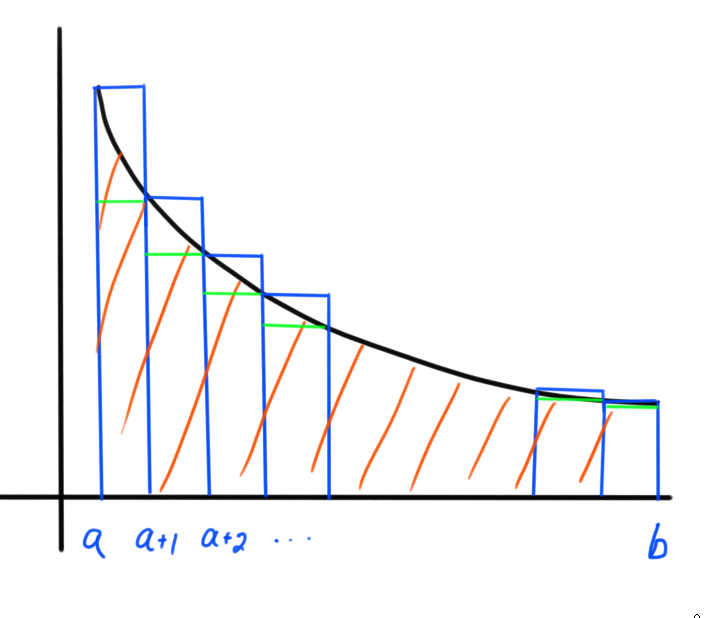
\includegraphics[scale=0.3]{integrals_and_sums}
     \end{figure}
    
    $\sum\limits_{k=a}^b f(k) - \int\limits_a^b \le \sum\limits_{k=a}^b - \sum\limits_{k=a-1}^b = f(a)$ (аналогично $f(b) = \sum\limits_{k=a}^b - \sum\limits_{k=a}^{b-1}$)

\end{proof}
\begin{theorem}[интегральный признак сходимости ряда]
    Пусть $f\!:[1, +\infty) \to \R$ неотрицательная, монотонно убывающая. 

    Тогда  $\sum\limits_{n=1}^\infty f(n)$ и  $\int\limits_1^\infty f(x) \mathrm{d}x$ ведут себя одинаково.
\end{theorem}
\begin{proof}
    По предыдущей теореме $S_n \coloneqq \sum\limits_{k=1}^n f(k) \ge \int\limits_1^n f(x)\mathrm{d}x \ge \sum\limits_{k=2}^n f(k) = S_n - f(1)$.

    Если ряд сходится, то $S_n$ --- ограничена  $\implies \int\limits_1^n f(x)\mathrm{d}x$ ограничена $\implies F(x) = \int\limits_1^x f$ --- ограничена $\implies \int\limits_1^\infty f(x)$ сходится.

    Если  $\int$ сходится $\implies \int\limits_1^n f$ --- ограничена  $\implies S_n$ --- ограничена  $\implies$ ряд сходится.
\end{proof}
\begin{example}
     \begin{enumerate}
         \item $\sum\limits_{n=1}^\infty \frac{1}{n^p}$, $p > 0$ (иначе члены ряда $\centernot \to 0$ и ряд расходится).\\
             $f(x) = \frac{1}{x^p}$. Монотонно убывает. $\sum \frac{1}{n^p}$ и $\int\limits_1^\infty \frac{\mathrm{d}x}{x^p}$ ведут себя одинаково: сходятся при  $p > 1$.
         \item $\sum\limits_{n=2}^\infty \frac{1}{n\ln n}$. $f(x) = \frac{1}{x\ln x}$ монотонно убывает. Поэтому $\int\limits_2^\infty \frac{\mathrm{d}x}{x\ln x}$ и $\sum\limits_{n=2}^\infty \frac{1}{n \ln n}$ ведут себя одинаково. 

             Там можно посчитать интеграл (разойдется).
    \end{enumerate}
\end{example}
\begin{consequence}
    \begin{enumerate}
        \item Если $a_n > 0$ и  $a_n = \mathcal{O}(\frac{1}{n^p})$ при $p > 1$ --- ряд  $\sum a_n$ --- сходится.
        \item Если  $a_n > 0$ и  $a_n \sim \frac{c}{n^p}$, то при $p > 1$ ряд  $\sum a_n$ --- сходится, а иначе расходится.
    \end{enumerate}
\end{consequence}
%END TICKET 59

\Subsection{Знакопеременные ряды}
\begin{definition}
    $\sum a_n$ --- сходится, но не абсолютно  $=$ ряд сходится условно.
\end{definition}
\begin{theorem}[Преобразование Абеля]
    $\sum\limits_{k=1}^n a_n b_n$.  $A_k \coloneqq a_1 + a_2 + \ldots + a_k$. Хочется заменить $a_n \to A_n$.

    Формулу сложнее запомнить, чем вывести, поэтому сначала выпишем её.
\end{theorem}
\begin{proof}
    \begin{align*}
        \sum_{k=1}^n a_k b_k &= \sum_{k=1}^n (A_k - A_{k-1})b_k = \sum_{k=1}^n A_kb_k - \sum_{j=2}^n A_{j-1}b_j \overset{k=j-1}{=} \sum_{k=1}^n A_kb_k - \sum_{k=1}^{n-1}A_kb_{k+1}  = \\ &= A_nb_n + \sum_{k=1}^{n-1}A_k(b_k - b_{k+1}).
    \end{align*}
\end{proof}
\begin{theorem}[Признак Дирихле]
    \begin{enumerate}
        \item $A_n$ (частичные суммы) --- ограничены ($|A_n| \le M$),
        \item $b_n$ монотонны,
        \item  $b_n \to 0$.
    \end{enumerate}
    Тогда $\sum\limits_{n=1}^\infty a_nb_n$ --- сходится.
\end{theorem}
\begin{proof}
    \begin{align*}
    S_n \coloneqq \sum_{k=1}^n a_k b_k = \underbracket{A_nb_n}_{\mathclap{\text{огр. на б.м.}}} + \sum\limits_{k=1}^{n-1}A_k(b_k-b_{k+1})
    \end{align*}
    Надо показать, что $\sum\limits_{k=1}^\infty A_k(b_k - b_{k+1})$ --- сходится. Для этого докажем, что ряд абсолютно сходится: $\sum\limits_{k=1}^\infty |A_k||b_k - b_{k+1}|$ --- сходится. 

    Мы знаем, что $\sum\limits_{k=1}^\infty |A_k||b_k - b_{k+1}| \le \sum\limits_{k=1}^\infty M \cdot |b_k - b_{k+1}| \overset{(*)}{=} M|\sum\limits_{k=1}^\infty (b_k - b_{k+1})| \le M|b_1|$.

    $(*)$ --- у нас постоянная монотонность, следовательно все слагаемые одного знака.
\end{proof}
\begin{theorem}[Признак Абеля]
    \begin{enumerate}
        \item Ряд $\sum\limits_{n=1}^\infty a_n$ --- сходится,
        \item $b_n$ --- монотонны,
        \item $b_n$ --- ограничены.
    \end{enumerate}
    Следовательно, $\sum\limits_{n=1}^\infty a_nb_n$ сходится.
\end{theorem}
\begin{proof}
    $2) + 3) \implies \exists \R \ni b \coloneqq \lim b_n$. Тогда  $\widetilde{b}_n \coloneqq b_n - b$ монотонны и  $\to 0$.

     $\sum\limits_{n=1}^\infty a_n$ --- сходится  $\implies A_n$ имеет предел  $\implies$  $A_n$ --- ограничены.

     Тогда  $\sum\limits_{n=1}^\infty a_n \widetilde{b}_n$ --- сходится  по признаку Дирихле. $\sum\limits_{n=1}^\infty a_n \widetilde{b}_n = \sum\limits_{n=1}^\infty a_n(b_n - b) \implies \sum\limits_{n=1}^\infty a_n b_n = b\underbracket{\sum\limits_{n=1}^\infty a_n}_{\mathclap{\text{по усл.}}} + \underbracket{\sum\limits_{n=1}^\infty a_n \widetilde{b}_n}_{\mathclap{\text{выяснили}}}$. 
\end{proof}
\begin{example}
    $\sum\limits_{n=1}^\infty \frac{\sin n)}{n^p}$ - сходится при $p > 0: a_n = \sin n, b_n = \frac{1}{n^p}, |A_n| \leq 2$.
\end{example}
\begin{example}
    $\sum\limits_{n=1}^\infty \frac{1}{n^3 \sin^2 n}$ - сходимость неизвестна.
\end{example}
\begin{definition}
    Знакочередующийся ряд $\sum\limits_{n=1}^\infty (-1)^{n-1}a_n$,  $a_n \ge 0$.
\end{definition}
\begin{theorem}[Признак Лейбница]
    Пусть есть ряд $\sum\limits_{n=1}^\infty (-1)^{n-1} a_n$.  $a_n \ge 0$ и монотонно стремится к 0.

    Тогда ряд $\sum\limits_{n=1}^\infty (-1)^{n-1} a_n$ сходится (по Дирихле: $a_n = (-1)^{n-1}, b_n = a_n$). Более того,  $S_{2n} \le S \le S_{2n+1}$.
\end{theorem}
\begin{proof}
    $S_{2n+2} = S_{2n} + a_{2n +1} - a_{2n+2} \ge S_{2n}$. $S_{2n+3} = S_{2n+1} - a_{2n+2} + a_{2n+3} \le S_{2n+1}$.

    $[0, S_1] \supset [S_2, S_3] \supset [S_4, S_5] \supset \ldots \supset [S_{2n}, S_{2n+1}] \supset \ldots$. $S_{2n+1} - S_{2n} = a_{2n+1} \to 0$.

    Пусть  $S$ их общая точка. Тогда  $\lim S_{2n} = \lim S_{2n+1} = S$.
\end{proof}

\begin{example}[Ряд Лейбница]
    \[
           \sum\limits_{n=1}^\infty \frac{(-1)^{n-1}}{n}
    .\] 
   \begin{align*}
       S_{2n}&=1-\frac{1}{2} + \frac{1}{3} - \frac{1}{4} + \ldots + \frac{1}{2n-1} - \frac{1}{2n} = H_{2n} - 2(\frac{1}{2} + \frac{1}{4} + \ldots + \frac{1}{2n}) = H_{2n} - H_n = \\ 
          &= \ln 2n+ \gamma + o(1) - (\ln n + \gamma + o(1)) = \ln 2 + o(1).
   \end{align*}

    Здесь заменили в изначальной сумме все отрицательные слагаемые на положительные и вычли их удвоенную сумму.
\end{example}
\begin{example}
    $1 - \frac{1}{2} - \frac{1}{4} + \frac{1}{3} - \frac{1}{6} - \frac{1}{8} + \frac{1}{5} - \frac{1}{10} - \frac{1}{12} + \ldots$.

    $\widetilde{S}_{3n} = (1 - \frac{1}{2} - \frac{1}{4}) + (\frac{1}{3} - \frac{1}{6} - \frac{1}{8}) + (\frac{1}{5} - \frac{1}{10} - \frac{1}{12}) + \ldots + (\frac{1}{2n - 1} - \frac{1}{4n-2} - \frac{1}{4n}) = \sum\limits_{k=1}^n(\frac{1}{4k - 2} - \frac{1}{4k}) = \frac{1}{2} \sum\limits_{n=1}^n (\frac{1}{2k-1} - \frac{1}{2k}) = \frac{S_{2n}}{2} \to \frac{\ln 2}{2}$.
\end{example}
\begin{definition}
    $\vphi\!: \N \to \N$ --- биекция $\sum\limits_{n=1}^\infty a_{\vphi(n)}$ --- перестановка ряда $\sum\limits_{n=1}^\infty a_n$.
\end{definition}
\begin{theorem}
    Если $\sum\limits_{n=1}^\infty a_n$ абсолютно сходится, то  $\sum\limits_{n=1}^\infty a_{\vphi(n)} = \sum\limits_{n=1}^\infty a_n$.
\end{theorem}
\begin{proof}
    \begin{enumerate}
        \item $a_n \ge 0$. $S_n \coloneqq \sum\limits_{k=1}^n a_k \le S \coloneqq \sum\limits_{k=1}^\infty a_k$.

            $\widetilde{S}_n \coloneqq \sum\limits_{k=1}^n a_{\vphi(k)} \le S_{\max{\vphi(1), \ldots, \vphi(n)}} \le S \implies \lim \widetilde{S}_n \le S \implies \widetilde{S} \le S$. Но $\phi$ - биекция и, т.к. любая перестановка не увеличивает сумму ряда, то можем сделать обратную перестановку и получим $S \le \widetilde{S} \implies S = \widetilde{S}$
        \item $a_n \in \R$.  $a_n = (a_n)_+ - (a_n)_-$, где $(a)_+ \coloneqq \max\{a, 0\}, (a)_- \coloneqq \max\{-a, 0\}$.  $|a_n| = (a)_- + (a)_+ \ge (a_n)_\pm \ge 0$.

            Если $\sum |a_n|$ --- сходится, то  $\sum\limits_{n=1}^\infty(a_n)_\pm $ --- сходится.  $\sum (a_{\vphi(n)})_+ = \sum (a_n)_+$ и  $\sum (a_{\vphi(n)})_- = \sum (a_n)_- \implies $ ряд сходится.
    \end{enumerate}
\end{proof}

\begin{remark}
    \begin{enumerate}
        \item Теорема верна в полном нормированном пространстве.
        \item В $\R^d$ верно обратное: если любая перестановка не меняет суммы, то ряд абсолютно сходится.
        \item Если ряд $a_n \in \R$ сходится условно, то  $\sum\limits_{n=1}^\infty (a_n)_+ = \sum\limits_{n=1}^\infty (a_n)_- = +\infty$.
             \begin{proof}
                Если $\sum (a_n)_+ < +\infty$, то  $\sum |a_n| = 2 \sum a_n - \sum (a_n)_+$ --- противоречие.

                 $|a_n| = 2(a_n)_+ - a_n$.
            \end{proof}
        \item Если $a_n \ge 0$, то $\sum a_{\vphi(n)} = \sum a_n$ верно и для расходящегося.
    \end{enumerate}
\end{remark}
\begin{theorem}[Теорема Римана]
    Пусть $\sum\limits_{n=1}^\infty a_n$ сходится условно, тогда  $\forall s \in \overline{\R}$ найдется такая перестановка, что  $\sum\limits_{n=1}^\infty a_{\vphi(n)} = s$.

    Так же существует перестановка, для которой нет суммы.
\end{theorem}
\begin{proof}
    Запишем сумму $a_1 + a_2 + \ldots$. Сотрем все отрицательные слагаемые: $b_1 + b_2 + \ldots = \sum (a_n)_+ = +\infty$. Сотрем все положительные: $c_1 + c_2 + \ldots = \sum (a_n)_- = +\infty$.
     \begin{enumerate}
         \item Случай $s \in \R$.  $b_1 + b_2 + \ldots + b_n > s \ge b_1 + b_2  + \ldots + b_{n-1}$.

             Теперь будем набирать $c_i$, пока сумма больше  $s$. Потом снова начнем набирать  $b$\ldots

             Обозначим за $S_i$ сумму на  $i$-ом шаге. Тогда знаем, что  $a_n \to 0$.  $S_1 > S \ge S_1 - b_{n_1}$, $S_2 + c_{m_1} \ge S > S_2$, $S_3 > S \ge S_3 - b_{n_2}$, $S_4 + c_{m_2} \ge S > S_4$.

             $S_{2n+1} > S \ge S_{2n+1} - b_{n_k}$. $\underbrace{S + b_{n_k}}_{\to s} \ge S_{2k+1} > \underbrace{S}_{\to s}$. 
         \item Случай $\pm \infty$.

             Очев + упражнение.
         \item Случай безпредела. 

             Ежу понятно.
    \end{enumerate}
\end{proof}
\begin{theorem}[Теорема Коши о произведении рядов]
    Пусть $A \coloneqq \sum\limits_{n=1}^\infty a_n$ и  $B \coloneqq \sum\limits_{n=1}^\infty b_n$ и ряды абсолютно сходятся.

    Тогда ряд, составленный из  $a_kb_n$ в произвольном порядке абсолютно сходится и его сумма  $AB$.
\end{theorem}
\begin{proof}
    $A^* \coloneqq \sum\limits_{n=1}^\infty |a_n|, A_n^* \coloneqq \sum\limits_{k=1}^n |a_k|$.  $A^*_n \le A^*, B_n^* \le B^*$.

    $S_m^*$ --- частичная сумма для ряда из  $|a_kb_j|$. $S_N \le (|a_1| + |a_2| + \ldots + |a_n|)(|b_1| + |b_2| + \ldots + |b_m|) = A_n^* B_m^* \le A^* B^*$, где $n$ --- максимальный индекс у  $a_k$ в слагаемом из  $S_N^*$, $m$ --- то же самое для  $b_k$.

    $S_N^*$ ограничены $\implies$ ряд абсолютно сходится. Тогда можем попереставлять ашки и бшки и посмотреть на табличку.

    $$
    \begin{matrix}
        a_1 b_1 & a_1 b_2 & a_1 b_3 & a_1 b_4 & \dots \\
        a_2 b_1 & a_2 b_2 & a_2 b_3 & a_2 b_4 & \dots \\
        a_3 b_1 & a_3 b_2 & a_3 b_3 & a_3 b_4 & \dots \\
        a_4 b_1 & a_4 b_2 & a_3 b_3 & a_4 b_4 & \dots \\
        \dots & \dots & \dots & \dots & \dots
    \end{matrix}
    $$

    Посмотрим на частичные суммы в квадратиках $i \times i$. $S_{n^2} = \sum\limits_{k=1}^n \sum\limits_{j=1}^n a_k b_j = \sum\limits_{k=1}^n a_k \sum\limits_{j=1}^n b_j = A_nB_n \to AB$.
\end{proof}

\begin{definition}
    $\sum\limits_{n=1}^\infty a_n$ и $\sum\limits_{n=1}^\infty b_n$ произведение этих рядов --- ряд  $\sum\limits_{n=1}^\infty c_n$, где  $c_n = a_1b_n + a_2b_{n-1} + a_3b_{n-2} + \ldots + a_nb_1$.
\end{definition}
\begin{theorem}[Теорема Мертенса]
    $A = \sum\limits_{n=1}^\infty a_n, B = \sum\limits_{n=1}^\infty b_n$ --- сходятся, причем один из них абсолютно.

    Тогда  $\sum\limits_{n=1}^\infty c_n$ --- сходится и его сумма  $AB$.
\end{theorem}
\begin{proof}
    Не доказывалось в курсе.
\end{proof}
\begin{remark}
    Абсолютной сходимости нет, важен порядок слагаемых.
\end{remark}
\begin{remark}
    Обычной сходимости не хватает.
\end{remark}
\begin{example}
    $\sum\limits_{n=1}^\infty \frac{(-1)^{n-1}}{\sqrt{n}}$ сходится по признаку Лейбница.

    $a_n = b_n = \frac{(-1)^{n-1}}{\sqrt{n}}$. \[c_n = (-1)^{n-1}(\underbrace{\frac{1}{\sqrt{n}} + \frac{1}{\sqrt{2}}\frac{1}{\sqrt{n-1}} + \ldots + \frac{1}{\sqrt{n}}1}_{\ge n \cdot \frac{1}{\sqrt{n}} \frac{1}{\sqrt{n}}}).\]
    А значит $|c_n| \ge 1$, а необходимое условие сходимости отсутствует. 
\end{example}
\begin{theorem}[Теорема Абеля]
    $A = \sum\limits_{n=1}^\infty a_n, B = \sum\limits_{n=1}^\infty b_n$ и  $C = \sum\limits_{n=1}^\infty c_n$ ---  произведение рядов.

    Если все три ряда сходятся, то  $AB=C$.
\end{theorem}
\begin{lemma}
    Пусть $x_n \to x$ и  $y_n \to y$. Тогда:
     \[
    \frac{x_1y_n + x_2y_{n-1} + \ldots + x_ny_1}{n} \to xy
    .\] 
\end{lemma}
\begin{proof}[Доказательство леммы]
    Случай $y=0$. Надо доказать, что $x_1y_n + \ldots + x_ny_1 = o(n)$. $|x_n| \le M, |y_n| \le M$. $\forall \eps > 0 \exists N\!: |y_n| \le \eps$ при $n \ge N$.

    Тогда в сумме все слагаемые с  $y_n$, где  $n \ge N$ будут $\le \eps M$, а первые $N$ ---  $\le M^2$. Тогда сумма $\frac{|\ldots|}{n} < \eps M + \frac{NM^2}{n} < 2\eps M$ при больших $n$.

    Случай  $y_n \equiv y$. Тогда сумма $\frac{\ldots}{n} = y \frac{x_1 + x_2 + \ldots + x_n}{n} \to xy$ по теореме Штольца.

    Общий случай: $y_n = y + \widetilde{y_n}, \widetilde{y_n} \to 0$. Тогда сумма с  $\widetilde{y_n}$ стремится к нулю, а, следовательно исходная стремится к  $xy$. Складываем и получаем что нужно.
\end{proof}
\begin{proof}[Доказательство теоремы]
    Рассмотрим $AB \leftarrow \frac{A_1 B_n + A_2 B_{n-1} + \ldots + A_nB_2}{n} = \frac{C_1 + C_2 + \ldots + C_n}{n} \to C$.

    Для доказательства равенства посчитаем количество вхождений слагаемых вида $a_i b_j$ в $C$ и $AB$. $c_{i+j}$ встречается $n - (i + j) + 1$ раз в $C_{i+j}$ и последующих и столько же раз в $A_k B_l$ при $k \ge i$ и $l \ge j$.
\end{proof}
\Subsection{Бесконечные произведения}
\begin{definition}
    $\prod\limits_{k=1}^\infty b_k$, сходящийся, если  $\exists \lim P_n$, он конечен и  $\neq 0$. $P_n$ - частичные произведения, аналогично суммам.
\end{definition}
\begin{example}
    \begin{enumerate}
        \item $\prod\limits_{k=2}^\infty \left(1-\frac{1}{k^2}\right)$. Оно очевидным образом равно $\frac{1}{2}$.
        \item $\prod_{n=1}^\infty(1 - \frac{1}{4n^2}) = \frac{1 \cdot 3 \cdot 3 \cdot 5 \cdot 5 \cdot 7 \cdot \ldots \cdot (2n-1)(2n+1)}{2^2 \cdot 4^2 \cdot 6^2 \cdot \dots \cdot (2n)^2 } = \frac{((2n-1)!!)^2(2n+1)}{((2n)!!)^2} \xrightarrow{\text{ф-ла Валиса}} \frac{2}{\pi}$
    \end{enumerate}
\end{example}
\begin{properties}
    \begin{enumerate}
        \item Добавление / выкидывание конечного числа ненулевых сомножителей не влияет на сходимость.
        \item Если  $\prod\limits_{k=1}^\infty b_k$ --- сходится, то  $\lim b_k = 1$.
             \begin{proof}
                $b_n = \frac{P_n}{P_{n-1}} \to \frac{P}{P} = 1$, так как $P \neq 0$ и  $\infty$.
            \end{proof}
        \item У сходящегося произведения начиная с некоторого места все множители $>0$. 
        \item  $\prod\limits_{n=1}^\infty b_n$ для  $b_n > 0$. 

             $\prod\limits_{n=1}^\infty b_n$ --- сходится  $\iff \sum\limits_{n = 0}^\infty \ln b_n$ --- сходится. Причем произведение --- $\exp$ от суммы.
\begin{proof}
    $P_n = \prod\limits_{k=1}^n b_k$.  $\ln P_n = \sum\limits_{k=1}^n \ln b_k \eqqcolon S_n$.

     $P_n$ имеет предел из  $(0; +\infty) \iff \ln P_n = S_n$ --- имеет конечный  $\lim \iff \sum \ln b_n$ --- сходящийся.
\end{proof}

    \end{enumerate}
\end{properties}
\begin{example}
    $\prod\limits_{n=1}^\infty \frac{p_n}{p_n - 1} = \prod\limits_{n=1}^\infty \sum\limits_{j=0}^\infty \frac{1}{p_n^j}$ --- где $p_n$ ---  $n$-ое простое число.

     $\prod\limits_{k=1}^n \frac{p_k}{p_k - 1} \ge H_n$.


     $\prod\limits_{k=1}^n \frac{p_k}{p_k - 1} = \prod\limits_{k=1}^n \frac{1}{1-\frac{1}{p_k}} > \prod\limits_{k=1}^n \sum\limits_{j=0}^n \frac{1}{p_k^j} = \sum \frac{1}{p_1^{\alpha_1} \ldots p_n^{\alpha_n}} > \sum\limits_{k=1}^n \frac{1}{k} = H_n \to \infty$.
\end{example}
\begin{theorem}
    $\sum\limits_{n=1}^\infty \frac{1}{p_n}$ --- расходится. Более того $\sum\limits_{k=1}^n \frac{1}{p_k} \ge \ln \ln n - 2$.
\end{theorem}
\begin{proof}
    $\sum\limits_{k=1}^n \frac{1}{1-\frac{1}{p_k}} > H_n \implies \sum\limits_{k=1}^n \ln(\frac{1}{1-\frac{1}{p_k}}) > \ln H_n > \ln \ln n$.

    Очевидно (по разложению $\ln(1 - x)$ по Тейлору), что $\ln(1-x) \ge -x -x^2$.

    Тогда $\sum\limits_{k=1}^n \ln(\frac{1}{1-\frac{1}{p_k}}) \le \sum\limits_{k=1}^n \frac{1}{p_k} + \underbrace{\sum\limits_{k=1}^n \frac{1}{p_k^2}}_{\le 2}$
\end{proof}
\begin{remark}
    \[
    \sum\limits_{k=1}^n \frac{1}{p_k} = \ln \ln n + O(1)
    .\] 
\end{remark}
\begin{exerc}
    \begin{enumerate}
        \item Доказать, что $S(k) = \sum\limits_{k < p \le k^2} \frac{1}{p} < \frac{4}{3}$.

            \textbf{Указание:} Посчитать количество чисел $\le k^2$, которые делятся на такие $p$.
        \item Доказать, что  $\sum\limits_{\mathclap{\substack{p \ge n\\p\text{ ---  простое}}}} \frac{1}{p} < 2 \ln \ln n + 4$.
    \end{enumerate}
\end{exerc}
\Subsection{Функциональные последовательности и ряды}
\begin{definition}
    $f, f_n\!: E \to \R$,  $f_n$ поточечно сходится к  $f$, если   $\forall x \in E\!: \lim\limits_{n \to \infty} f_n(x) = f(x)$.

    В кванторах:  $\forall x \in E \forall \eps > 0 \exists N = N(x, \eps)\!: \forall n \ge N |f_n(x) - f(x)| < \eps$.
\end{definition}
\begin{definition}
    $f_n$ равномерно сходится к  $f$ на  $E$  $f_n \rightrightarrows f$ на $E$:
     \[
    \forall \eps > 0 \exists N=N(\eps) \forall n \ge N \forall x \in E\!: |f_n(x) - f(x)| < \eps
    .\] 
\end{definition}
\begin{remark}
    Из равномерной сходимости следует поточечная.
\end{remark}
\begin{example}
    $f_n(x) = x^n$,  $E = (0, 1)$.

     $\lim f_n(x) = \lim x^n = 0$. $f(x) \equiv 0 \implies $  $f_n$ поточечно сходится к  $f$. При этом, если взять  $x > \sqrt[n]{\eps}$, то мы проиграли, следовательно равномерной сходимости нет.
\end{example}
\begin{remark}
    Равномерная сходимость на графике --- графики $f_n$ начиная с некоторого места попадают в полоску графика  $f$.
\end{remark}
\begin{figure}[!h]
	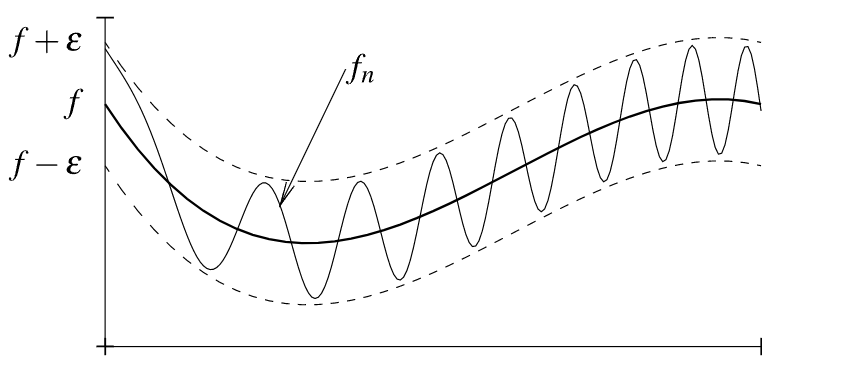
\includegraphics[scale=0.45]{uniform_conv}
\end{figure}
\begin{theorem}
    $f_n, f\!:E \to \R$. 

    Тогда  $f_n \underset{E}{\rightrightarrows} f \iff \sup\limits_{x \in E} |f_n(x) - f(x)| \to 0$
\end{theorem}
\begin{proof}
    $\Rightarrow$: $f_n \underset{E}{\rightrightarrows} f \iff \forall \eps > 0 \exists N \forall n \ge N\!: \forall x \in E |f_n(x) - f(x)| < \eps$. Из части c $\forall x \in E$ как раз прямо и следует условие на  $\sup$.\\
    $\Leftarrow$: $\lim\limits_{n \to \infty} \sup\limits_{x \in E} |f_n(x) - f(x)| = 0 \iff \forall \eps > 0 \exists N \forall n \ge N \sup\limits_{x \in E}|f_n(x) - f(x)| < \eps$. Из супремума следует $\forall x \in E |f_n(x) - f(x)| < \eps$.\\
    Здесь мы пользовались тем, что $\sup|f_n(x) - f(x)| \geq |f_n(x) - f(x)|$.
\end{proof}
\begin{consequence}
\begin{enumerate}
    \item Если $\forall x \in E\quad |f_n(x) - f(x)| \le a_n$ и $\lim a_n = 0$, то $f_n \underset{E}{\rightrightarrows} f$.
    \item Если  $x_n \in E\!: f_n(x_n) - f(x_n) \centernot \to 0$, то нет равномерной сходимости  $f_n \underset{E}{\rightrightarrows} f$.
\end{enumerate}
\end{consequence}
\begin{proof}
    \begin{enumerate}
        \item $\implies 0 \le \sup\limits_{x \in E} |f_n(x) - f(x)| \le a_n \to 0 \implies \sup \to 0 \implies f_n \underset{E}{\rightrightarrows}f$.
        \item $\sup\limits_{x \in E} |f_n(x) - f(x)| \ge |f_n(x_n)  - f(x_n)| \centernot \to 0 \implies \sup \centernot \to 0 \implies$ нет равномерной сходимости. Здесь $x_n$~--- какая-то конкретная точка.
    \end{enumerate}
\end{proof}
\begin{example}
    $E=(0, 1), f(x) \equiv 0, f_n(x) = x^n$. $x_n = 1 - \frac{1}{n}$, $f_n(x_n) - f(x_n) = \left(1-\frac{1}{n}\right)^n \to \frac{1}{e} \neq 0 \implies$ нет равномерной сходимости.
\end{example}
\begin{definition}
    $g_n \!: E \to \R$ --- равномерно ограничена, если найдется  $M$, такой что\\$|g_n(x)| \le M \quad \forall x \in E\quad\forall n$
\end{definition}
\begin{statement}
    Произведение равномерно ограниченной и равномерно сходящейся к нулю равномерно~--- сходится к нулю.
\end{statement}
\begin{proof}
    $g_n$ --- равномерно ограничена,  $|g_n(x)| \le M, f_n(x) \rightrightarrows 0$, $\sup\limits_{x \in E} |f_n(x)| \to 0$.

     $\sup\limits_{x \in E} |f_n(x)g_n(x)| \le M \sup \to 0 \implies f_ng_n \rightrightarrows 0$.
\end{proof}
\begin{remark}
    \begin{enumerate}
        \item $f_n \underset{E}{\rightrightarrows} f \iff f_n - f \underset{E}{\rightrightarrows} 0$.
        \item  Если $f_n \rightrightarrows f, g_n \rightrightarrows g \implies \alpha f_n + \beta g_n \rightrightarrows \alpha f + \beta g$.
    \end{enumerate}
\end{remark}
\begin{theorem}[Критерий Коши для равномерной сходимости последовательности функций]
    $f_n\!: E \to \R$ тогда  $f_n$ равномерно сходится к некоторой функции  $\iff \forall \eps > 0 \exists N \forall m, n \ge N \forall x \in E |f_n(x) - f_m(x) | < \eps$.
\end{theorem}
\begin{proof}
    $\implies$:  $f_n \underset{E}{\rightrightarrows} f$ $\iff$ $\forall \eps > 0 \exists N \begin{array}{l} \forall n \ge N \forall x \in E |f_n(x) - f(x)| < \frac{\eps}{2} \\ \forall m \ge N \forall x \in E |f_m(x) - f(x)| < \frac{\eps}{2} \end{array}$. 

    $\forall m, n \ge N \forall x \in E |f_n(x) - f_m(x)| \le |f_n(x) - f(x)| + |f_m(x) - f(x)| < \frac{\eps}{2} + \frac{\eps}{2} = \eps$.

    $\Leftarrow$:  $\forall \eps > 0 \exists N \forall m, n \ge N_e \forall x \in E\quad |f_n(x) - f_m(x)| < \eps$. Зафиксируем $x \in E$. Если  $m_n \ge N_\eps$, то знаем заклинание $\implies f_n(x)$ --- фундаментальная последовательность  $\implies$ она имеет конечный предел. Пусть $f(x) \coloneqq \lim\limits_{n \to \infty} f_n(x)$.

    Тогда  $\forall \eps > 0 \exists N \forall m \ge n \ge N \forall x \in E \quad |f_n(x) - f_m(x)| < \eps$ --- критерий Коши. Устремим тут $m \to \infty$. Тогда  $\forall \eps > 0 \exists N \forall n \ge N \forall x \in E |f_n(x) - f(x)| \le \eps \implies f_n$ равномерно сходится к $f$.
\end{proof}
\begin{definition}
    Пространство $C(K)$,  $K$ --- компакт. 

     $C(K) \coloneqq \{f\!: K \to \R \land f \text{ непрерывна во всех точках}\}$ --- векторное пространство.

      $f, g\!: K \to \R, (\alpha f+\beta g)(x) \coloneqq \alpha f(x) + \beta g(x)$.

      Можно завести норму  $\|f\|_{C(K)} \coloneqq \max\limits_{x \in K} |f(x)|$ --- нормированное пространство.

      Убедимся, что это действительно норма. Интересно только неравенство треугольника: $\|f+g\| = |f(x_0) + g(x_0)| \le |f(x_0)| + |g(x_0| \le \|f\| + \|g\|$.
\end{definition}
\begin{definition}
    Пространство $l^\infty(E)$.

     $l^\infty(E) \coloneqq \{f\!: E \to \R \land f\text{ --- ограничена}\}$ --- векторное пространство.

     $\|f\|_{l^\infty(E)} \coloneqq \sup_{x \in E}|f(x)|$~--- нормированное пространство.
\end{definition}
\begin{remark}
    $C(K) \subset l^{\infty}(K)$.
\end{remark}
\begin{theorem}
    $l^\infty(E)$ --- полное пространство.
\end{theorem}
\begin{proof}
    $f_n$ --- фундаментальная последовательность  $\iff \forall \eps > 0 \exists N \forall m, n \ge N \sup\limits_{x \in E} |f_n(x) - f_m(y)| = \|f_n - f_m\| < \eps \implies \forall \eps > 0 \exists N \forall m, n \ge N \forall x \in E |f_n(x) - f_m(x)| < \eps \implies f_n$ --- равномерно сходится на $E \implies \sup_{x \in E} |f_n(x) - f(x)| = \|f_n - f\|_{l^\infty(E)} \to 0$. Надо проверить, что  $f \in l^\infty(E)$.

     $f_n(x) \le \underbrace{|f(x) - f_n(x)}_{\le \|f - f_n\| < 1} + \underbrace{|f_n(x)|}_{\le \|f_n\|}$.
\end{proof}
\begin{theorem}
    $f_n, f\!: E \to \R, a \in E, f_n \underset{E}{\rightrightarrows} f$ и  $f_n$ непрерывна в точке $a$. Тогда  $f$ непрерывна в точке  $a$.
\end{theorem}
\begin{proof}
    Берем $\eps > 0$. Найдем  $N$, такой что  $\forall n \ge N \forall x \in E |f_n(x) - f(x)| < \eps$.

    $|f(x) - f(a)| \le \underbrace{|f(x) - f_N(x)|}_{< \eps} + \underbrace{|f_N(x) - f_N(a)|}_{< \eps, \text{ если } |x-a| < \delta} + \underbrace{|f_N(a) - f(a)|}_{< \eps} < 3\eps$.

    $\exists \delta > 0 \forall |x-a| < \delta\quad |f_N(x)- f_N(a)| < \eps \implies f$ --- непрерывна в $a$.
\end{proof}
\begin{consequence}[Теорема Стокса-Зайделя]
    $f_n \underset{E}{\rightrightarrows} f$ и  $f_n$ непрерывна во всех точках  $E \implies f$ непрерывна во всех точках из  $E$. Пользуемся предыдущей теоремой для каждой точки.
\end{consequence}
\begin{theorem}
    $C(K)$ --- полное.
\end{theorem}
\begin{lemma}
    $(X, \rho)$ --- полное метрическое пространство, $Y \subset X$ --- замкнутое  $\implies (Y, \rho)$ --- полное. 
\end{lemma}
\begin{proof}[Доказательство леммы]
    Возьмем $y_n \in Y$ --- фундаментальная последовательность в  $Y \implies$ она фундаментальна в $X \implies \exists y_* \in X\!: y_* = \lim y_n \implies y_*$ ---  предельная точка  $Y \implies y_* \in Y$.
\end{proof}
\begin{proof}[Доказательство теоремы]
    $C(K)$ --- замкнутое подпространство  $l^\infty(K)$.  $\sup\limits_{x \in K}|f_n(x) - f(x)| =\|f_n - f\|_{l^\infty(K)} \to 0$. Тогда если $f_n \in C(K), f_n \underset{K}{\rightrightarrows} f \implies f \in C(K)$ по т.Стокса-Зайделя.
\end{proof}
\begin{definition}
    $u_n\!: E \to \R$.  $\sum\limits_{n=1}^\infty u_n(x)$ --- функциональный ряд.

     $S_n(x) \coloneqq \sum\limits_{k=1}^n u_k(x)\!: E \to \R$ --- частичная сумма ряда.

     Если  $S_n$ поточечно сходится к  $S$, то ряд сходится поточечно.

     Если $S_n \underset{E}{\rightrightarrows} S$, то ряд равномерно сходится на  $E$.
\end{definition}
\begin{definition}
    Если ряд $\sum\limits_{n=1}^\infty u_n(x)$ сходится поточечно, то  $r_n(x) \coloneqq \sum\limits_{k=n+1}^\infty u_k(x)$ --- остаток (хвост) ряда.
\end{definition}
\begin{theorem}
    Ряд $\sum\limits_{k=1}^\infty u_n(x)$ сходится равномерно на  $E \iff r_n \underset{E}{\rightrightarrows} 0$.
\end{theorem}
\begin{proof}
    $S_n \underset{E}{\rightrightarrows} S \iff S - S_n \rightrightarrows 0$. ($S - S_n = r_n$).
\end{proof}
\begin{remark}
    Необходимые условия равномерной сходимости. Если $\sum\limits_{n = 1}^{\infty} u_n(x)$ равномерно сходится, то  $u_n \rightrightarrows 0$.
\end{remark}
\begin{proof}
    Равномерная сходимость $\implies S_n \rightrightarrows S \implies S_n - S_{n-1} \rightrightarrows S - S = 0$.
\end{proof}
\begin{remark}
    Если $x_n \in E\!: \underbracket{u_n(x_n) \centernot \to 0}_{\mathclap{\text{нет равномерной сходимости } \to 0}}$, то $\sum\limits_{n=1}^\infty u_n(x)$ не может равномерно сходиться.
\end{remark}
\begin{remark}
    Из расходимости ряда $\sum\limits_{n=1}^\infty u_n(x_n)$ ничего не следует.

    $u_n(x) = \begin{cases} \frac{1}{n} & x \in (\frac{1}{n+1}, n] \\ 0 & \text{иначе} \end{cases}.$ 

    $x_n = \frac{1}{n} \implies u_n(x_n) = \frac{1}{n}$ и ряд $\sum u_n(x_n)$ --- расходится.

    Но ряд $\sum\limits_{n=1}^\infty u_n(x)$ равномерно сходится.  $0 \le r_n(x) \le \frac{1}{n+1}. r_n \rightrightarrows 0$.
\end{remark}
\begin{theorem}[Критерий Коши для равномерной сходимости ряда]
    $u_n\!: E \to \R$. Ряд  $\sum\limits_{n=1}^\infty u_n(x)$ равномерно сходится на  $E \iff$
     \[
    \forall \eps > 0 \exists N \forall m, n \ge N \forall x \in E |\sum\limits_{k=n+1}^m u_k(x)| < \eps.
    .\] 
\end{theorem}
\begin{proof}
    $\sum u_n(x)$ равномерно сходится  $\iff S_n(x) \coloneqq \sum\limits_{k=1}^n u_k(x)$ равномерно сходится  $\iff \forall \eps > 0 \exists N \forall m > n \ge N \forall x \in E |S_m(x) - S_n(x)| < \eps$, а эта разность как раз то, что надо.
\end{proof}

\begin{theorem}[Признак сравнения]
   $u_n, v_n\!: E \to \R$,  $|u_n(x)| \le v_n(x) \quad \forall x \in E, \forall n$.

   Если $\sum\limits_{n=1}^\infty v_n(x)$ сходится равномерно на  $E$, то ряд  $\sum\limits_{n=1}^\infty u_n(x)$ равномерно сходится на  $E$.
\end{theorem}
\begin{proof}
    Применим к левой части критерий Коши: $\forall \eps > 0 \exists N \forall m > n \ge N \forall x \in E \quad |\sum\limits_{k=n+1}^m u_k(x)| \le \sum\limits_{k=n+1}^m |u_k(x)|\le \sum\limits_{k=n+1}^m v_k(x)< \eps$. Откуда получаем, что ряд $\sum\limits_{k=1}^\infty u_k(x) $ равномерно сходится на  $E$.
\end{proof}
\begin{consequence}
    \begin{enumerate}
        \item Если $\sum |u_n(x)|$ сходится равномерно на  $E$, то  $\sum u_n(x)$ сходится равномерно на  $E$. 
        \item Признак Вейерштрасса. Если  $|u_n(x)| \le a_n \quad \forall x \in E \forall n$ и ряд $\sum a_n$ --- сходится, то  $\sum u_n(x)$ сходится равномерно на  $E$.
    \end{enumerate}
\end{consequence}
\begin{example}
    $\sum\limits_{n=1}^\infty \frac{\sin nx}{n^2}$ равномерная сходимость на $\R$.

     $\left| \frac{\sin nx}{n^2}\right| \le \frac{1}{n^2}$. $\sum\limits_{n=1}^\infty \frac{1}{n^2}$ --- сходится.
\end{example}
\begin{remark}
    Ряд может сходиться равномерно, но не абсолютно $\sum\limits_{n=1}^\infty \frac{(-1)^n}{n}$

    Ряд сходится абсолютно, но не сходится равномерно $\sum\limits_{n=1}^\infty x^n$ при $x \in (-1, 1)$.

    Ряд сходится абсолютно, ряд сходится равномерно, но ряд $\sum |u_n(x)|$ сходится неравномерно.
\end{remark}
\begin{theorem}[Признак Дирихле]
    $a_n, b_n\!: E \to \R$.
     \begin{enumerate}
         \item $\left|\sum\limits_{k=1}^n a_k(x)\right| \le M \quad \forall x \in E \forall n$.
         \item $b_n(x)$ монотонно при любом фиксированном $x \in E$.
         \item  $b_n \rightrightarrows 0$.
    \end{enumerate}

    Тогда ряд $\sum\limits_{n=1}^\infty a_n(x)b_n(x)$ сходится равномерно на  $E$.
\end{theorem}
\begin{proof}
   $S_n(x) \coloneqq \sum\limits_{k=1}^n a_k(x)b_k(x) = A_n(x)b_n(x) + \sum\limits_{k=1}^{n-1}A_k(x)(b_k(x) - b_{k+1}(x))$, где $A_n$ --- частичная сумма  $a$.

   $A_nb_n \rightrightarrows 0$, так как  $A_n$ равномерно ограничена и  $b_n \rightrightarrows 0$.

   Докажем, что ряд $\sum\limits_{k=1}^\infty A_k(x)(b_k(x) - b_{k+1}(x))$ равномерно сходится.

   $|A_k(x)| |b_k(x) - b_{k+1}(x)| \le M|b_k(x) - b_{k+1}(x)| \eqqcolon v_k(x)$. Надо доказать, что $\sum\limits_{k=1}^\infty v_k(x)$ равномерно сходится, то есть  $\sum\limits_{k=1}^\infty |b_k(x) - b_{k+1}(x)|$ равномерно сходится. $\sum\limits_{k=1}^n |b_k(x) - b_{k+1}(x)| = |\sum\limits_{k=1}^n (b_k(x) - b_{k+1}(x))| = b_1(x) - b_n(x) \rightrightarrows b_1(x)$
\end{proof}
\begin{theorem}[Признак Абеля]
    $a_n, b_n\!: E \to \R$.
     \begin{enumerate}
         \item $\sum\limits_{n=1}^\infty a_n(x)$ --- равномерно сходится.
         \item  $b_n(x)$ монотонно при любом фиксированном  $x \in E$.
         \item  $b_n(x)$ равномерно ограничена.
    \end{enumerate}

    Тогда $\sum\limits_{n=1}^\infty a_n(x)b_n(x)$ сходится равномерно на  $E$.
\end{theorem}
\begin{proof}
    $\sum\limits_{k=n+1}^{n+p} a_k(x)b_k(x) = \sum\limits_{k=1}^p a_{n+k}(x)b_{n+k}(x) = (A_{n+p}(x) - A_p(x))b_{n+p}(x)+\sum\limits_{k=1}^{p-1} (A_{n+k}(x) - A_{k}(x))(b_{n+k}(x) - b_{n+k+1}(x))$.
    
    $\sum\limits_{k=1}^{m} a_{n+k}(x) = A_{n+m}(x) - A_n(x)$.

    $A_n(x) \rightrightarrows A(x) \implies \forall \eps > 0 \exists N \forall m, n \ge N \forall x \in E\!: |A_n(x) - A_m(x)| < \eps$.

    Тогда $|A_{n+p}(x) - A_n(x)| < \eps$ и  $|A_{n+k}(x) - A_n(x)| < \eps$.

     $|\sum\limits_{k=n+1}^{n+p} a_k(x)b_k(x)| \le \underbrace{|A_{n+p}(x) - A_n(x)|}_{\mathclap{< \eps}} \cdot \underbrace{|b_{n+p}(x)|}_{\le M} + \sum\limits_{k=1}^{p-1} \underbrace{|A_{n+k}(x)-A_n(x)}_{\le \eps}|b_{n+k}(x) - b_{n+k+1}(x)| \le \eps M + \eps\sum\limits_{k=1}^{p-1}|b_{n+k}(x) - b_{n+k+1}(x)| = \eps M + \eps|\sum\limits_{k=1}^{p-1}(b_{n+k}(x) - b_{n+k+1}(x))| \le \eps M + \eps \cdot 2M = 3M\eps$.
     
     По критерию Коши для $\sum a_nb_n$ он равномерно сходится.
\end{proof}
\begin{theorem}[Признак Лейбница]
    $b_n\!: E \to \R$,  $b_n \rightrightarrows 0, b_n(x)$ монотонна при любом фиксированном  $x \in E$. Тогда ряд  $\sum\limits_{k=1}^\infty (-1)^k b_n(x)$ равномерно сходится на  $E$.
\end{theorem}
\begin{proof}
    $a_n(x) = (-1)^n$,  $\sum\limits_{k=1}^n a_k(x) = 0$ или  $-1  \implies $ равномерно ограничен. Применим признак Дирихле.
\end{proof}
\begin{example}
    $\sum\limits_{n=1}^\infty \frac{(-1)^n}{n}x^n$ при $x \in (0, 1)$.

    Ряд абсолютно сходится $\forall x \in (0, 1)\!: \left| \frac{(-1)^n}{n}x^n\right| \le x^n$.

    Ряд сходится равномерно $b_n(x) = \frac{x^n}{n} \rightrightarrows 0, 0 \le b_n(x) \le \frac{1}{n}, x_n(x) \searrow$.

    $\sum\limits_{n=1}^\infty \left|\frac{(-1)^n}{n}x^n \right| = \sum\limits_{n=1}^\infty \frac{x^n}{n}$.

    Нет равномерной сходимости. $\sum\limits_{k=n}^{2n} \frac{x^k}{k} \ge n \frac{x^{2n}}{2n} = \frac{x^{2n}}{2} \to \frac{1}{2e}$, $x = 1 - \frac{1}{2n}$.
\end{example}
\begin{theorem}[Признак Дини]
    $0 \le u_n \in C(K)$, $K$ --- компакт и  $S_x \coloneqq \sum\limits_{n=1}^\infty u_n(x) \in C(k)$. Тогда ряд сходится равномерно на  $K$.
\end{theorem}
\begin{proof}
    $r_n(x) = S(x) - S_n(x) \in C(K), S(x) - S_n(x) = \sum\limits_{k=n+1}^\infty u_k(x), 0 \le r_{n+1} \le r_n(x)$.

    Надо доказать, что $r_n \underset{K}{\rightrightarrows} 0$.  $r_n(x_n) = \sup\limits_{x \in K} r_n(x) \to 0$ для некоторого $x_n \in K$.

    От противного. Пусть нет стремления к нулю.  $r_{n_k}(x_{n_k}) \ge \eps$, $x_{n_k} \in K$. Выберем сходящуюся подпоследовательность  $x_{m_k} \to x_* \in K$.

     $r_{m_k}(x_{m_k}) \ge \eps$. $x_{m_k} \to x_*$. Тогда  $r_n(x_{m_k}) \ge r_{n+1}(x_{m_k}) \ge r_{n+2}(x_{m_k}) \ge \ldots \ge r_{m_k}(x_{m_k}) \ge \eps$, при этом $r_n(x_{m_k}) \to r_n(x_*) \implies r_n(x_*) \ge \eps \quad \forall x$. Но $r_n(x_*) \to 0$. Противоречие.
\end{proof}

\Subsection{Свойства равномерно сходящихся последовательностей и рядов}
\begin{theorem}
    $f_n, f\!: E \to \R$,  $a$ --- предельная точка  $E$,  $f_n \rightrightarrows f$ на  $E$ и  $\lim\limits_{x \to a} f_n(x) \eqqcolon b_n \in \R$. Тогда  $\lim b_n, \lim\limits_{x \to a} f(x)$ существуют, конечны и равны.

    В частности, $\lim\limits_{x \to a} \lim\limits_{n \to \infty} f_n(x) = \lim\limits_{n \to \infty} \lim_{x \to a} f_n(x)$.
\end{theorem}
\begin{proof}
    Запишем Критерий Коши:
    \[\forall \eps > 0 \exists N\forall m, n \ge N \forall x \in E\!: |f_n(x) - f_m(x)| < \eps.\] 
    Устремим в этом неравенстве $x \to a$ (тогда $f_n(x) \to b_n, f_m(x) \to b_m$):
    \[
    \forall \eps > 0 \exists N\forall m, n \ge N \forall x \in E\!: |b_n - b_m| \le \eps 
    .\] А это критерий Коши для последовательности $b_n \implies \lim b_n = b \in \R$.

    Остается показать, что $\lim\limits_{x \to a} f(x) = b$. Честно проверим. Что такое $|f(x) - b|$? Это  $\le |f_n(x) - f(x)| + |b_n - f_n(x)| + |b-b_n|$. Мы знаем, что $b_n \to b \implies |b-b_n|$ при  $n \ge N_1$ не больше $\eps$. При  $n \ge N_2$ $|f_n(x) - f(x)| M \eps$. 

    Тогда, взяв  $N \coloneqq \max(N_1, N_2)$, получаем $|f(x) - b| < 2\eps + |b_n - f_n(x)|$. Но оставшаяся разность стремится к нулю при  $x \to a$. Тогда можно выбрать $\delta$-окрестность, чтобы эта разность  была меньше $\eps$. Следовательно,  $|f(x) - b| < 3\eps$.
\end{proof}
\begin{theorem}
    $u_n\!: E \to \R$,  $\sum\limits_{n=1}^\infty u_n(x)$ равномерно сходится и $\lim\limits_{x \to a}u_n(x) = c_n$, $a$ --- предельная точка.
\\
   Тогда,  $\lim\limits_{x \to a} \sum\limits_{n=1}^\infty u_n(x) = \sum\limits_{n=1}^\infty c_n = \sum\limits_{n=1}^\infty \lim\limits_{x \to a}u_n(x)$ и ряд сходится.
\\
   То есть, в случае равномерной сходимости ряда мы можем менять предел суммы.
\end{theorem}
\begin{proof}
    $f_n(x) \coloneqq \sum\limits_{k=1}^n u_k(x) \rightrightarrows f(x) = \sum\limits_{n=1}^\infty u_n(x)$, $b_n = \lim\limits_{x \to a} f_n(x) \overset{(*)}{=} \lim\limits_{x \to a} \sum\limits_{k=1}^n u_k(x) = \sum\limits_{k=1}^n \lim\limits_{x \to a} u_k(x) = \sum\limits_{k=1}^n c_k$.
\\
    Тогда $\exists \lim b_n$, то есть ряд $\sum\limits_{n=1}^\infty c_n$ сходится и $\lim\limits_{n \to \infty} b_n = \lim\limits_{x \to a} f(x) = \lim\limits_{x \to a} \sum\limits_{n=1}^\infty u_n(x)$.
\\
     $(*)$ --- тут конечная сумма, поэтому все переходы конечны.
\end{proof}
\begin{consequence}
    Если $u_n$ непрерывны в точке  $a$ и  $\sum\limits_{n=1}^\infty u_n(x)$ равномерно сходится, то  $\sum u_n(x)$ непрерывна в точке  $a$.
\end{consequence}
\begin{proof}
    $c_n = u_n(a)$.
\end{proof}
\begin{theorem}
    Пусть $f_n \in C[a, b]$ и  $f_n \rightrightarrows f$ на  $[a, b]$, $c \in [a,b]$.

    Тогда $\int\limits_c^x f_n(t)\dt \rightrightarrows \int\limits_c^x f(t)\dt$. В частности $\lim\limits_{n \to \infty} \int\limits_c^x f_n(t)\dt = \int\limits_c^x \lim\limits_{n \to \infty} f_n(t)\dt$

\end{theorem}
\begin{proof}
    $F_n(x) \coloneqq \int\limits_c^x f_n(t) \dt$. Тогда  $|F_n(x) - F(x)| = \left|\int\limits_c^xf_n(t)\dt - \int\limits_c^x f(t)\dt\right| \le \int\limits_c^x |f_n(t) - f(t)| \dt \le |x-c|\max\limits_{t \in [c, x]} |f_n(t) - f(t)| \le (b-a)\sum\limits_{t \in [a, b]} |f_n(t) - f(t)|$, но по свойству равномерной сходимости $\sup \to 0$. Значит равномерная сходимость есть.
\end{proof}
\begin{consequence}
    $u_n \in C[a, b]$ и  $\sum\limits_{n=1}^\infty u_n(x)$ равномерно сходится, то $\int\limits_c^x \sum\limits_{n=1}^\infty u_n(t)\dt = \sum\limits_{n=1}^\infty \int\limits_c^x u_n(t)\dt$.
\end{consequence}
\begin{proof}
    $\int\limits_c^x\sum\limits_{k=1}^n u_k(t)\dt = \sum\limits_{k=1}^n \int\limits_c^x u_k(t)\dt$. А дальше можно просто устремить к бесконечности по предыдущей теореме.
\end{proof}
\begin{remark}
    Поточечной сходимости не хватает. Пример: $f_n(x) nxe^{-nx^2}$ на  $[0, 1]$.  $f_n(x) \xrightarrow{n \to \infty} 0$. То $\int\limits_0^1 f_n(x) \dx = \int\limits_0^1 nxe^{-nx^2}\dx = \frac{1}{2} \int\limits_0^1 e^{-nx^2} \mathrm(nx^2) = -\frac{e^{-nx^2}}{2} \Big|_0^1 = \frac{1-e^{-n}}{2} \to \frac{1}{2} \neq 0 = \int\limits_0^1 f(x)\dx$.
\end{remark}
\begin{theorem}
    $f_n \in C^1[a, b], c \in [a, b], f_n(c) \to A$ и  $f_n' \rightrightarrows g$ на $[a, b]$. 
    
    Тогда  $f_n \rightrightarrows f$ на  $[a, b]$,  $f \in C^1[a, b]$ и $f' = g$.

    В частности, $\lim\limits_{n \to \infty} f_n'(x) = (\lim\limits_{n \to \infty} f_n(x))'$
\end{theorem}
\begin{proof}
    $\int\limits_c^x g(t)\dt = \int\limits_c^x \lim\limits_{n \to \infty} f_n'(t) \dt \overset{(*)} = \lim_{n \to \infty} \int\limits)c^x f_n'\dt = \lim\limits_{n \to \infty} (f_n(x) - f_n(c)) = \lim\limits_{n \to \infty} f_n(x) - \lim\limits_{n \to \infty} f_n(c) = f(x) - A$. $(*)$ --- предыдущая теорема.

    Тогда $f(x) = A + \int\limits_c^x g(y)\dt \implies f \in C^1[a, b]$ и  $f'(x) = g(x)$.

    Осталось понять, что  $f_n \rightrightarrows f$.

     $f_n(x) = \int\limits_c^x f_n'(t)\dt + f_n(c)$,  $f(x) = \int\limits_c^x g(t)\dt + A$.

     Мы знаем, что  $\int\limits_c^x f_n'(t)\dt \rightrightarrows \int\limits_c^xg(t)\dt$, а $f_n(c) \to A \implies f_n(c) \rightrightarrows A$.
\end{proof}
\begin{consequence}
    $u_n \in C^1[a, b]$ и  $\sum\limits_{n=1}^\infty u'_n(x)$ равномерно сходится на  $[a, b)$,  $\sum\limits_{n=1}^\infty u_n(c)$ сходится. 

    Тогда  $\sum\limits_{n=1}^\infty u_n(x)$ равномерно сходится к дифференцируемой функции и $\left(\sum\limits_{n=1}^\infty u_n(x)\right)' = \sum\limits_{n=1}^\infty u_n'(x)$.
\end{consequence}
\begin{proof}
    $f_n(x) = \sum\limits_{k=1}^n u_k(x) \in C^1[a, b]$ и  $f_n'(x) = \sum\limits_{k=1}^n u_k'(x) \rightrightarrows \sum\limits_{k=1}^\infty u_k'(x) \eqqcolon g(x)$.

     $f_n' \rightrightarrows g$ и  $f_n(c)$ сходятся.

     Тогда по теорема  $f_n \rightrightarrows f$,  $f$ --- дифференцируемая функция и  $f' = g$.

     То есть мы поняли, что $\left(\sum\limits_{n=1}^\infty u_n(x)\right)' = g(x) = \sum\limits_{n=1}^\infty u_n'(x)$. 
\end{proof}
\begin{remark}
    Равномерной сходимости исходных функций недостаточно. Пример: $\sum\limits_{n=1}^\infty \frac{\sin nx}{n^2}$ равномерно сходится: $\left| \frac{\sin nx}{n^2} \right| \le \frac{1}{n^2}$ и признак Вейерштрасса. $\sum\limits_{n=1}^\infty \left(\frac{\sin nx}{n^2}\right)' = \sum\limits_{n=1}^\infty \frac{\cos nx}{n}$ расходится в $x = 0$.
\end{remark}
\Subsection{Степенные ряды}
\begin{definition}
    $a_n \in \CC, z, z_o \in \CC$,  $\sum\limits_{n=0}^\infty a_n(z-z_0)^n$ --- степенной ряд. Здесь $a_n$ --- закрепленная последовательность,  $z_0$ --- константа. Поэтому можно делать формулы проще и использовать  $w = z - z_0$.
\end{definition}
\begin{theorem}
    Пусть ряд $\sum\limits_{n=0}^\infty a_nz^n$ сходится при некотором  $z = z_0$. Тогда ряд абсолютно сходится  $\forall z\!: |z| < |z_0|$.
\end{theorem}
\begin{proof}
    $\sum\limits_{n=0}^\infty a_n z_0^n$ --- сходящийся $\implies |a_nz_0^n| \to 0 \implies |a_nz_0^n| \le M$.

    Тогда скажем, что $|a_nz^n| = |a_nz_0^n| \cdot \left|\frac{z}{z_0}\right|^n \le M \left|\frac{z}{z_0}\right|^n$.
\end{proof}
\begin{consequence}
    Если ряд $\sum\limits_{n=0}^\infty a_nz^n$ расходится при  $z=z_0$, то он расходится  $\forall z\!: |z| > |z_0|$.
\end{consequence}
\begin{definition}
    $R$ --- радиус сходимости ряда, если ряд  $\sum a_nz^n$  сходится $\forall z\!: |z| < R$ и расходится  $\forall z\!: |z| > R$.
\end{definition}
\begin{theorem}
    Радиус сходимости существует $\in [0, +\infty]$ и  $R = \frac{1}{\varlimsup \sqrt[n]{|a_n|}}$ --- формула Коши-Адамара (Hadamard).
\end{theorem}
\begin{proof}
    Докажем, что $R = \frac{1}{\varlimsup \sqrt[n]{a_n}}$ подходит. Для этого применим к этому ряд признак Коши с $K \coloneqq \varlimsup \sqrt[n]{|a_n|} = \varlimsup |z| \sqrt[n]{|a_n|} = \frac{|z|}{R}$. Признак Коши: $K < 1 \implies$ ряд сходится, если  $K > 1 \implies$ ряд расходится.
\end{proof}
\begin{example}
    \begin{enumerate}
        \item $\sum\limits_{k=0}^\infty \frac{z^n}{n!}$. $R = \frac{1}{\varlimsup \sqrt[n]{\frac{1}{n!}}} = +\infty$. Ряд сходится всегда.
        \item $\sum\limits_{n=0}^\infty n!z^n$,  $R = \frac{1}{\varlimsup \sqrt[n]{n!}} = 0$. Ряд сходится при $z = 0$.
        \item  $\sum\limits_{n=1}^\infty \frac{z^n}{n^p}$, $R = \frac{1}{\varlimsup \sqrt[n]{\frac{1}{n^p}}} = 1$. Ряд точно сходится при $|z| < 1$. Ряд при  $|z| \le 1$ ряд сходится. А вот при $p=1$ ряд расходится при  $p=1$ и сходится при  $z = -1$.
    \end{enumerate}
\end{example}
\begin{definition}
    $R$ --- радиус сходимости  $\sum\limits_{n=0}^\infty a_n(z-z_0)^n$.

    Круг $\{z \in \CC \mid |z-z_0| < R\|$ --- круг сходимости.
\end{definition}
\begin{theorem}
    $R$ --- радиус сходимости ряда  $\sum\limits_{n=0}^\infty a_nz^n$ и  $0 < r < R$.

    Тогда ряд  $\sum a_nz^n$ сходится равномерно при  $|z| \le r$.
\end{theorem}
\begin{proof}
    $\sum\limits_{n=0}^\infty a_nr^n$ --- абсолютно сходится  $\implies \sum\limits_{n=0}^\infty |a_n| r^n < +\infty$.

    Если $|z| \le r$, то $|a_nz^n| \le |a_n|r^n \implies$ равномерно сходится по признаку Вейерштрасса.  
\end{proof}
\begin{consequence}
    Сумма степенного ряда --- непрерывная в круге сходимости функция.
\end{consequence}
\begin{proof}
    Проверим непрерывность в точке $z = w$.

     $|w| < r < R \implies$ ряд сходится равномерно в круге  $|z| \le r \implies$ сумма ряда непрерывна в круге $|z| < r \implies$ в точке $z = w$ есть непрерывность. 
\end{proof}
\begin{theorem}[Теорема Абеля]
    Пусть $\sum\limits_{n=0}^\infty a_nz^n$ сходится при  $z = R$, где  $R$ --- радиус сходимости. 

    Тогда ряд сходится равномерно на $[0; R]$ и его сумма непрерывна на  $[0; R]$.

    В том числе $\lim\limits_{x \to R-} \sum\limits_{n=0}^\infty a_nx^n = \sum\limits_{n=0}^\infty a_nR^n$.
\end{theorem}
\begin{proof}
    $\sum\limits_{n=0}^\infty a_nx^n = \sum\limits_{n=0}^\infty a_nR^n\left(\frac{x}{R}\right)^n$.

    $\sum\limits_{n=0}^\infty a_nR^n$ --- равномерно сходящийся.  $\left(\frac{x}{R}\right)^n$ монотонна и равномерно ограничена $\xRightarrow{\text{пр. Абеля}} \sum\limits_{n=0}^\infty a_nx^n$ равномерно сходится  $\implies f(x) \coloneqq \sum\limits_{n=0}^\infty a_nx^n$ непрерывна на  $[0; R]$.
\end{proof}
\begin{lemma}
    $x_n, y_n \ge 0$. $\lim x_b \in (0; +\infty)$.

    Тогда  $\varlimsup x_ny_n = \lim x_n \varlimsup y_n$.
\end{lemma}
\begin{proof}
    Берем $x_{n_k}y_{n_k} \to \varlimsup x_n y_n = b$.

    $x_{n_k} \to a \implies y_{n_k} \to \frac{b}{a} \le c \coloneqq \varlimsup y_n \implies b \le ac$.

    Берем $y_{n_k} \to c \implies x_{n_k}y_{n_k} \to ac \le b \implies b = ac$.
\end{proof}
\begin{consequence}
    $\sum\limits_{n=0}^\infty a_n z^n, \sum\limits_{n=0}^\infty a_n \frac{z^{n+1}}{n+1}$ и $\sum\limits_{n=1}^\infty na_n z^{n-1}$ имеют одинаковые радиусы сходимости.
\end{consequence}
\begin{proof}
    Заметим, что $\sum\limits_{n=0}^\infty a_n \frac{z^{n+1}}{n+1}$ и $\sum\limits_{n=0}^\infty a_n \frac{z^{n}}{n+1}$ имеют одинаковые радиусы сходимости.

    Заметим, что  $\sum\limits_{n=0}^\infty n a_n z^{n-1}$ и  $\sum\limits_{n=0}^\infty n a_n z^{n}$ имеют одинаковые радиусы сходимости.

    $R_1 = \frac{1}{\varlimsup \sqrt[n]{|a_n|}}$, $R_2 = \frac{1}{\varlimsup \sqrt[n]{\frac{|a_n|}{n+1}}}$, $R_3 = \frac{1}{\varlimsup \sqrt[n]{|a_n| \cdot n}}$.
\end{proof}

\begin{theorem}[о почленном интегрировании степенного ряда $\sum\limits_{n=0}^\infty a_n(x-x_0)^n = f(x)$]
    $R$ --- его радиус сходимости. Тогда  $\int\limits_{x_0}^y f(x)\dx = \sum\limits_{n=1}^\infty a_n \frac{(y-x_0)^{n+1}}{n+1}$, где $|y-x_0| < R$.
\end{theorem}
\begin{proof}
    Ряд $\sum a_n(x-x_0)^n$ равномерно сходится при $|x-x_0| \le |y-x_0|$. На $[x_0, y]$ есть равномерная сходимость. Тогда
\begin{align*}
    \sum\limits_{x_0}^y \sum\limits_{n=0}^\infty a_n(x-x_0)^n \dx = \sum\limits_{n=0}^\infty \int\limits_{x_0}^y a_n(x-x_0)^n \dx = \sum\limits_{n=0}^\infty a_n \frac{(y-x_0)^{n+1}}{n+1}.
\end{align*}
\end{proof}
\begin{definition}
    $f\!: E \to \CC$,  $z_0 \in \Int E$.

    $f$ --- дифференцируема в точке  $z_0$, если $f(z) = f(z_0) + k(z-z_0) + o(z-z_0)$  при $z \to z_0$.
\end{definition}
\begin{definition}
    $f'(z_0) = \lim\limits_{z \to z_0} \frac{f(z) - f(z_0)}{z - z_0}$.
\end{definition}
\begin{remark}
    Дифференцируемость $\iff$ $f'(z_0)$ конечна и $k = f'(z_0)$.
\end{remark}
\begin{theorem}
    $f(z) = \sum\limits_{n=0}^\infty a_n(z-z_0)^n, |z-z_0| < R$ --- радиус сходимости.

    Тогда $f$ бесконечно дифференцируема в круге сходимости и  $f^{(m)}(z) = \sum\limits_{n=m}^\infty a_n n (n-1) \ldots (n - m + 1)(z-z_0)^{n-m}$
\end{theorem}
\begin{proof}
    Ряд справа имеет тот же радиус сходимости.

    $\sum\limits_{n=1}^\infty na_n(z - z_0)^{n-1} \implies$ при $|z-z_0| \le r < R$ он равномерно сходится.

    \begin{align*}
        f'(z) &= \lim\limits_{w \to z} \frac{f(w) - f(z)}{w - z} = \lim\limits_{w \to z} \frac{\sum\limits_{n=0}^\infty a_nw^n - \sum\limits_{n=0}^\infty a_nz^n}{w - z} = \lim\limits_{w \to z} \sum\limits_{n=0}a_n \frac{w^n - z^n}{w - z}  = \\
              &= \lim\limits_{w \to z} \sum\limits_{n=1}^\infty a_n(w^{n-1} + w^{n-2}z + \ldots + wz^{n-2} + z^{n-1}) \overset{?}{=} \sum\limits_{n=1}^\infty \lim\limits_{w \to z} a_n(w^{n-1} + \ldots z^{n-1}) = \sum\limits_{n=1}^\infty a_n n z^{n-1}
\end{align*}
Разберемся с вопросом: $|a_n(w^{n-1} + \ldots + z^{n-1})| \le |a_n| n r^{n-1}$, а $\sum\limits_{n=1}^\infty n|a_n| r^{n-1}$ сходится.
\end{proof}
\begin{theorem}
    Разложение функции в степенной ряд единственно. 

    Если $f(z) = \sum\limits_{n=0}^\infty a_n(z-z_0)^n$, то $a_b = \frac{f^{(n)}(z_0)}{n!}$.
\end{theorem}
\begin{proof}
    $f^{(m)}(z_0) = a_m m(m-1)\ldots 1 = m!a_m$.
\end{proof}
\begin{definition}
    $f$ аналитическая в точке  $x_0$, если в окрестности $x_0$ $f(x) = \sum\limits_{n=0}^\infty \frac{f^{(n)}(x_0)}{n!}(x-x_0)^n$
\end{definition}
\begin{remark}
    Бесконечно дифференцируемая функция $\centernot\implies$ аналитичность. 
\end{remark}
\begin{example}
    $f(x) = \begin{cases} 0, & x = 0\\e^{-\frac{1}{x^2}}, & x \neq 0 \end{cases}$. Это бесконечно дифференцируемая функция. 

    Тут абоба по индукции.
\end{example}
\begin{example}
    $e^z \coloneqq \sum\limits_{n=0}^\infty \frac{z^n}{n!}$, $\cos z \coloneqq \sum\limits_{n=0}^\infty \frac{(-1)^n z^{2n}}{(2n)!}$, $\sin z \coloneqq \sum\limits_{n=0}^\infty \frac{(-1)^n z^{2n+1}}{(2n+1)!}$.
\end{example}
\begin{exerc}
    $e^{iz} = \cos z + i\sin z$,  $\cos^2 z + \sin^2 z = 1, e^w e^z = e^{w+z}$.

    $\cos z = \frac{e^{iz} + e^{-iz}}{2}$, $\sin z = \frac{e^{iz} - e^{-iz}}{2}$.
\end{exerc}
\begin{example}
    При $|x| < 1$.

    $\ln(1+x) = \sum\limits_{n=1}^\infty \frac{(-1)^{n-1}x^n}{n}$.

    $\arctg x = \sum\limits_{n=0}^\infty \frac{(-1)^n x^{2n+1}}{2n+1}$.
\end{example}
\begin{proof}
    $(\ln (1+x))' = \frac{1}{1+x} = \sum\limits_{n=0}^\infty (-1)^n x^n$.

    $\ln(1+y) = \int\limits_0^y \frac{\dx}{1+x} = \int\limits_0^y \sum\limits_{n=0}^\infty (-1)^n x^n = \sum\limits_{n=0}^\infty (-1)^n \frac{y^{n=1}}{n+1}$.

     $(\arctg x)' = \frac{1}{1+x^2} = \sum\limits_{n=0}^\infty (-1)^n x^{2n}$.

     $\arctg y = \int\limits_0^y \frac{\dx}{1+x^2} = \int\limits_0^y \sum\limits_{y=0}^\infty (-1)^n x^{2n} \dx = \sum\limits_{n=0}^\infty (-1)^n \frac{y^{2n+1}}{2n+1}$.
\end{proof}
\begin{example}
    $(1+x)^p = \sum\limits_{n=0}^\infty \frac{p(p-1)\ldots(p-n+1)}{n!}x^n$ при $|x| < 1$.
\end{example}
\begin{proof}
    $(1+x)^p = \sum\limits_{k=0}^n \frac{p(p-1)\ldots (p-k+1)}{k!}x^k + \frac{1}{n!}\int\limits_0^x p(p-1)\ldots (p-n)(1+t)^{p-n-1}(x-t)^n \dt$. 

    Посчитаем $\frac{c_{n+1}}{c_n} = \frac{1}{n} \cdot \ldots = \frac{p-n}{n} \frac{\int\limits_0^x (1+t)^{p-n}(x-t)^{n-1}\frac{x-t}{1+t} \dt}{\int\limits_0^x (1+t)^{p-n} (x_t)^{n-1}\dt}$.

    Тогда $\left| \frac{x-t}{1+t} \right| \le |x|$. А значит отношение $\le \frac{p - n}{n}|x| \to |x| \le 1$.
\end{proof}
\begin{example}
    Частный случай при  $p = -\frac{1}{2}$. 
    \begin{align*}
        \frac{1}{\sqrt{1+x}} = 1 + \sum\limits_{n=1}^\infty \frac{(-1)^n\frac{1}{2} \cdot \frac{3}{2} \cdot \frac{5}{2} \cdot \ldots \cdot (n-\frac{1}{2})}{n!}x^n = 1 + \sum \limits_{n=1}^\infty \frac{(2n-1)!!(-1)^n}{2^nn!}x^n = 1 + \sum\limits_{n=1}^\infty \frac{\binom{2n}{n}(-1)^n}{4^n}x^n
    \end{align*}
\end{example}
\begin{example}
    \begin{align*}
        \arcsin x = \sum\limits_{n=0}^\infty \frac{\binom{2n}{n}}{4^n} \cdot \frac{2^{n+1}}{2n+1}.
    \end{align*}
\end{example}
\begin{proof}
     \begin{align*}
        \frac{1}{\sqrt{1-x^2}} = 1 + \sum\limits_{k=1}^\infty \frac{\binom{2n}{n}}{4^n}x^{2n}
    \end{align*}
    Но мы знаем, что $\arcsin y = \int\limits_0^y \frac{\mathrm{d}x}{\sqrt{1-x^2}} = y + \sum\limits_{n=1}^\infty \frac{\binom{2n}{n}}{4^n} \frac{y^{2n+1}}{2n+1}$.
\end{proof}
